% In this section the available data sets must be presented. The term dataset
% refers to any type of information source, for example web services for
% geolocation fall into this category. In addition, all necessary data
% manipulation processes, such as cleaning and enrichment with external sources,
% must be presented and discussed.

Il Dataset in esame contiene all'incirca 1.39 milioni di prodotti e per ognuno
di essi fornisce le caratteristiche seguenti.
\subsubsection{Price}
\textbf{Price} rappresenta il prezzo di vendita dell'articolo, ovvero la
variabile target della regressione. Il suo valore medio è di circa \$26, con un
minimo pari a \$0, un massimo di \$2009 e una deviazione standard di circa \$38.
Analizzando meglio la distribuzione si nota che in generale i prezzi sono
relativamente bassi in quanto inferiori a \$29 per il 75\% dei prodotti.
\subsubsection{Train id}
\textbf{Train\_id} rappresenta l'identificativo del prodotto nell'elenco.
\subsubsection{Name}
\textbf{Name} è il nome del prodotto sotto forma di dato non strutturato.
% todo dato non strutturato. meglio testo?
\subsubsection{Shipping}
\textbf{Shipping} rappresenta di chi, tra venditore e acquirente, sono a carico
le spese di spedizione: il valore 1 significa "a carico del
venditore", 0 invece dell'acquirente.

I costi di spedizione risultano ben distribuiti tra venditori e acquirenti: il
45\% dei prodotti è spedito a carico del venditore (Shipping=1), mentre il
restante 55\% a carico dell'acquirente (Shipping=0).

Ci si potrebbe aspettare che i prodotti spediti a carico del venditore abbiano
prezzi più elevati; tuttavia, almeno per quanto riguarda l'intero dataset in
esame, è vero il contrario.

Infatti il prezzo medio dei prodotti spediti a carico degli acquirenti, circa
\$30, è superiore a quello dei prodotti restanti, circa \$22.

% spese di spedizione sono incluse nel prezzo? todo

\subsubsection{Item condition}
\textbf{Item\_condition\_id} rappresenta lo stato del prodotto; questo valore
varia da 1 a 5. Il valore più frequente è 1, mentre 4 e 5 sono i più rari. La
Kaggle challenge non ne fornisce una descrizione dettagliata sul significato. Si
può supporre che il valore 1, il più frequente, identifichi la condizione
migliore, mentre il valore 5 la condizione peggiore. Tuttavia, alla luce dei
prezzi medi per ogni condizione, la supposizione sembra essere errata: i
prodotti in condizione 5 hanno mediamente il prezzo maggiore, quelli in
condizione 4, invece, il prezzo minore; infine la differenza nel prezzo medio
degli articoli nelle condizioni 1,2 e 3 risulta molto lieve.
\subsubsection{Category Name}
\textbf{Category\_name}
% todo dire che abbiamo splittato in 3 le categorie

rappresenta la categoria di prodotto a cui appartiene l'articolo. Nel dataset
sono presenti 1287 categorie univoche e tra ognuna di esse si vede una categoria
principale/generale, seguita da due o più sottocategorie più specifiche (ad
esempio: Women/Tops \& Blouses/T-Shirts). Inoltre, ci sono 6327 articoli che non
hanno una categoria assegnata. Infine, analizzando le dieci categorie più
popolari, si nota che l'abbigliamento femminile è molto popolare su Mercari.
Infatti, di queste prime dieci categorie 5 sono di abbigliamento femminile;
Anche il trucco e l'elettronica sono categorie molto quotate.


rappresenta la categoria di prodotto a cui appartiene l'articolo. Nel dataset
sono presenti 1287 categorie univoche, ad esempio \textit{"Women/Tops \&
Blouses/T-Shirts"}, ed è facilmente osservabile una sorta di gerarchia di
sottocategorie dalla più generica alla più specifica.

Inoltre, circa 6000 articoli non hanno nessuna categoria assegnata, mentre analizzando categorie più numerose, si nota come l'abbigliamento
femminile sia molto popolare su Mercari; 5 categarie nelle top 10 sono infatti
di abbigliamento femminile. Trucco ed elettronica ricoprono anch'essi posizioni
rilevanti tra le categorie più quotate.
\subsubsection{Brand Name}
\textbf{Brand\_name} rappresenta il marchio dell'articolo; nel dataset sono
presenti 4809 valori differenti e più di 600 mila valori mancanti che
corrispondono a poco meno della metà dei prodotti totali.
\subsubsection{Item Description}
\textbf{Item\_description} rappresenta la descrizione del prodotto sotto forma
di dato non strutturato. Nel dataset sono presenti 4 istanze senza descrizione e
circa 82 mila con la stringa "no description yet".
Inoltre, non sembra esistere una relazione lineare tra lunghezza delle
descrizioni e prezzo, in quanto l'indice di correlazione di Pearson è prossimo a
zero; 0.048 per l'esattezza.

Analizzando le word cloud ottenute dai bigrammi delle descrizioni dopo aver
suddiviso i prodotti in quattro fasce di prezzo (figure \ref{fig:100},
\ref{Fig:50_100}, \ref{fig:30_50} e \ref{Fig:minore_30}) si riescono a notare delle differenze sulle coppie parole più frequenti, identificabili perchè
di dimensioni più grandi.

Infatti, nella wordcloud dei prodotti con prezzo superiore a \$100 (Figura
\ref{fig:100}) sono molto frequenti bigrammi che danno informazioni sulle buone
condizioni dei prodotti, ad esempio:  100 authentic, great condition e good
condition. Al diminuire del prezzo questi bigrammi diventano meno frequenti;
aumentano invece i bigrammi relativi a descrizioni mancanti.

\begin{figure}[H]
   \begin{minipage}{0.48\textwidth}
     \centering
     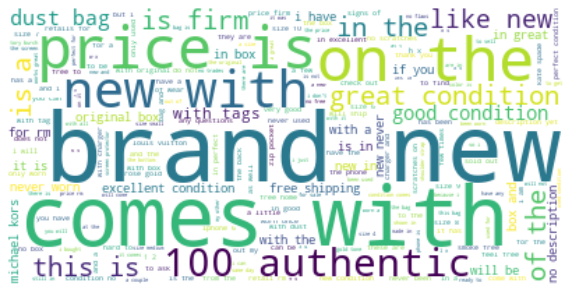
\includegraphics[width=.9\linewidth]{maggiore_100}
	\caption{Word Cloud contenente i bigrammi ottenuti dalle descrizioni dei prodotti con prezzo maggiore o uguale a 100}
	\label{fig:100}   
	\end{minipage}\hfill
   \begin{minipage}{0.48\textwidth}
     \centering
     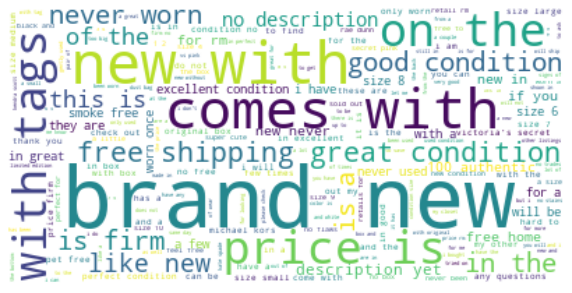
\includegraphics[width=.9\linewidth]{50_100}
     \caption{Word Cloud contenente i bigrammi ottenuti dalle descrizioni dei prodotti con prezzo maggiore di 50 e minore di 100}
     \label{Fig:50_100}
   \end{minipage}
\end{figure}

\begin{figure}[H]
   \begin{minipage}{0.48\textwidth}
     \centering
     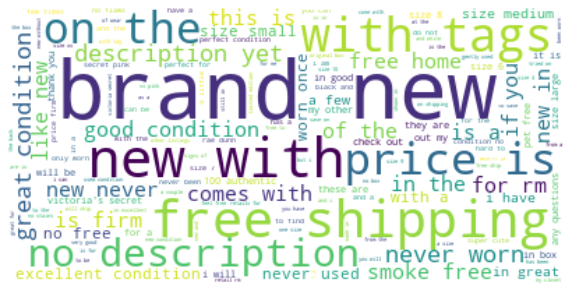
\includegraphics[width=.9\linewidth]{30_50}
	\caption{Word Cloud contenente i bigrammi ottenuti dalle descrizioni dei prodotti con prezzo maggiore di 30 e minore o uguale a 50}
	\label{fig:30_50}   
	\end{minipage}\hfill
   \begin{minipage}{0.48\textwidth}
     \centering
     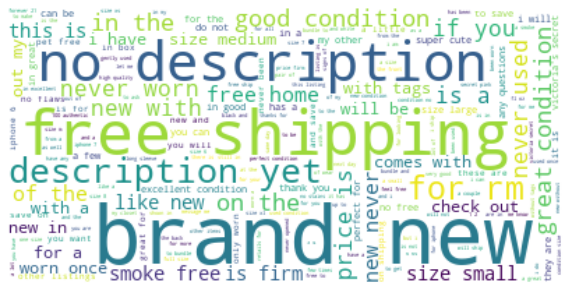
\includegraphics[width=.9\linewidth]{minore_30}
     \caption{Word Cloud contenente i bigrammi ottenuti dalle descrizioni dei prodotti con prezzo minore o uguale a 30}
     \label{Fig:minore_30}
   \end{minipage}
\end{figure}
\subsubsection{Pulizia Dataset}
Dal dataset sono stati eliminati tutti i prodotti con prezzi minori di cinque e maggiori di 2000 poichè sul sito ufficiale di Mercari è specificato che i prezzi possono essere impostati solo nell'intervallo [5,2000] (fonte: \url{https://www.mercari.com/us/help_center/article/69}).
Durante la fase di analisi si è scoperta la presenta di valori mancanti nei campi: item\_description, brand\_name e category\_name, questi valori sono stati rimpiazzati con il valore NA.
Inoltre, è stato effettuato un trattamento dei dati (cito paper sul text preprocessing) non strutturati convertendoli tutti in minuscolo, sono state sostituite le descrizioni mancanti con il valore NA (anche quando era presente la stringa "no description yet").
Sui dati testuali è stata effettuata una fase di lemmatizzazione (perchè usa vocabolario su cui tagliare le parole e cito articolo). Successivamente, sulle nuove parole ottenute è stata effettuata una fase di pulizia di questi campi non strutturati eliminando le stopwords, la punteggiatura, tutti i caratteri di lunghezza pari a 1 che non sono numeri (è stato deciso di mantenere tutti i numeri poichè molte descrizioni senza di essi perdono di significato) e sono state eliminate le emoji.


I valori del campo category\_name sono stati codificati in interi tramite la tecnica label encoding.

% todo: coefficiente di correlazione di  pearson?
% todo: piccole analisi come correlazioni sono da mettere qui? oppure nella
% sezione dopo?
% todo: far trasparire che abbiamo valutato entrambi gli approcci di text
% cleaning o no
